\documentclass[border=6pt]{standalone}
\usepackage{tikz}
\usetikzlibrary{calc, arrows.meta}

\definecolor{red-10}{HTML}{ef5350}   % #ef5350
\definecolor{yellow-10}{HTML}{ffca28}  % #ffca28
\definecolor{teal}{HTML}{1de8b5} % #1de8b5
\definecolor{gray-900}{HTML}{212529} % #212529
\definecolor{gray-500}{HTML}{98978b} % #98978b
\definecolor{black}{HTML}{000000} % #000000


\begin{document}
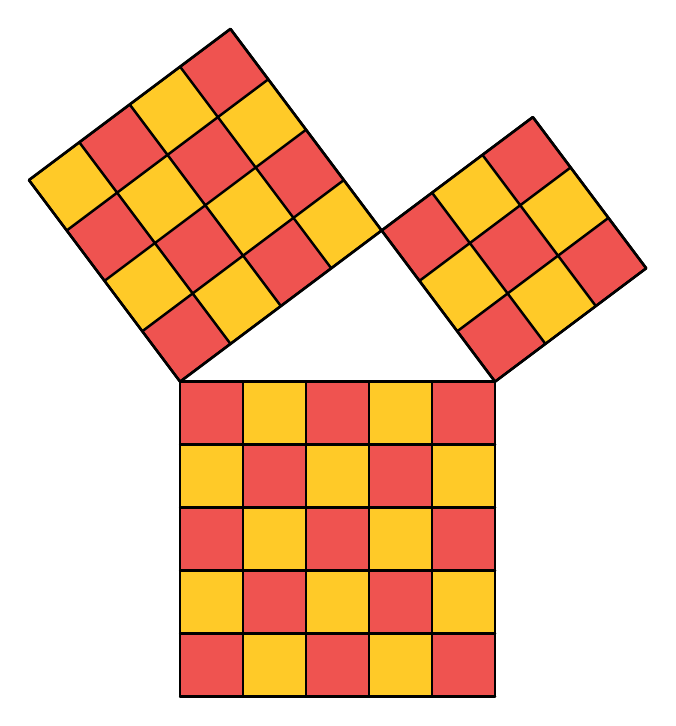
\begin{tikzpicture}[scale=0.8, line cap=round, line join=round, >=Stealth, every node/.style={font=\small}, rotate=-143.13]

% Tam giác vuông 3-4-5
\coordinate (A) at (0,0); 
\coordinate (B) at (4,0); 
\coordinate (C) at (0,3);

% Hàm vẽ caro đỏ-vàng xen kẽ
\newcommand{\CheckerSquare}[4]{%
  % #1: góc trái dưới, 
  % #2: độ dài cạnh (đơn vị),
  % #3: góc xoay, 
  % #4: hướng (1 ra ngoài, -1 vào trong)
  \begin{scope}[shift={#1}, rotate=#3, scale=#4]
    \foreach \i in {0,...,#2} {
      \foreach \j in {0,...,#2} {
        \ifnum\i<#2
          \ifnum\j<#2
            \pgfmathtruncatemacro{\isEven}{mod(\i+\j,2)}
            \ifnum\isEven=0
              \fill[red-10] (\i,\j) rectangle ++(1,1);
            \else
              \fill[yellow-10] (\i,\j) rectangle ++(1,1);
            \fi
          \fi
        \fi
      }
    }
    \draw[black, line width=0.9pt] (0,0) grid (#2,#2);
    \draw[black, line width=0.9pt] (0,0) rectangle (#2,#2);
  \end{scope}
}

% Hình vuông trên cạnh AB bốn đơn vị
\CheckerSquare{(0,-4)}{4}{0}{1}

% Hình vuông trên cạnh AC 3 đơn vị 
\CheckerSquare{(-3,0)}{3}{0}{1}

% Hình vuông trên cạnh huyền BC 5 đơn vị 
\CheckerSquare{(0,3)}{5}{-36.87}{1}

% Vẽ tam giác vuông lần nữa
% \draw [white] (A)--(B)--(C)--cycle;
% \draw[fill=white, draw=teal-50, line width=1.2pt] (A)--(B)--(C)--cycle;

% Chú thích cạnh
% \node[below] at ($(A)!0.5!(B)$) {$4$};
% \node[left]  at ($(A)!0.5!(C)$) {$3$};
% \node[above right] at ($(B)!0.5!(C)$) {$5$};

%Ký hiệu góc vuông tại A
% \draw (0.6,0)--(0.6,0.6)--(0,0.6);

\end{tikzpicture}
\end{document}
